%%%% Proceedings format for most of ACM conferences (with the exceptions listed below) and all ICPS volumes.
\documentclass[sigconf]{acmart}

\usepackage{listings} % code formatting
\lstset{
  basicstyle=\ttfamily,
  columns=fullflexible,
  breaklines=true,
}
\usepackage{graphicx} % images
\usepackage{subcaption} % subfigures
\usepackage{multicol}

% Copyright
% \setcopyright{none}
%\setcopyright{acmcopyright}
%\setcopyright{acmlicensed}
\setcopyright{rightsretained}
%\setcopyright{usgov}
%\setcopyright{usgovmixed}
%\setcopyright{cagov}
%\setcopyright{cagovmixed}

% DOI
\acmDOI{}

% ISBN
\acmISBN{}

%Conference
\acmConference[REBLS'18]{SPLASH Boston}{November 2018}{Boston, Massachusetts USA}
\acmYear{2018}
\copyrightyear{2018}

\acmArticle{}
\acmPrice{}

\begin{document}
\title{Explicitly Comprehensible Functional Reactive Programming}

% \author{Steven Krouse}
% \email{steveykrouse@gmail.com}

% % The default list of authors is too long for headers.
% \renewcommand{\shortauthors}{S. Krouse}

\begin{abstract}
Functional Reactive programs written in The Elm Architecture are difficult to comprehend without reading every line of code. A more modular architecture would allow programmers to understand a small piece without reading the entire application. This paper shows how higher-order and cyclic streams, as demonstrated with the Reflex library, can improve comprehensibility.\end{abstract}

\begin{CCSXML}
<ccs2012>
<concept>
<concept_id>10011007.10011006.10011008.10011009.10011012</concept_id>
<concept_desc>Software and its engineering~Functional languages</concept_desc>
<concept_significance>500</concept_significance>
</concept>
<concept>
<concept_id>10011007.10011006.10011008.10011024.10011028</concept_id>
<concept_desc>Software and its engineering~Data types and structures</concept_desc>
<concept_significance>300</concept_significance>
</concept>
<concept>
<concept_id>10011007.10011006.10011008.10011024.10011036</concept_id>
<concept_desc>Software and its engineering~Patterns</concept_desc>
<concept_significance>300</concept_significance>
</concept>
<concept>
<concept_id>10011007.10011006.10011008.10011024.10011038</concept_id>
<concept_desc>Software and its engineering~Frameworks</concept_desc>
<concept_significance>300</concept_significance>
</concept>
</ccs2012>
\end{CCSXML}

\ccsdesc[500]{Software and its engineering~Functional languages}
\ccsdesc[300]{Software and its engineering~Data types and structures}
\ccsdesc[300]{Software and its engineering~Patterns}
\ccsdesc[300]{Software and its engineering~Frameworks}

\keywords{functional reactive programming, elm, reflex}

\maketitle

\section{Introduction}

Today software projects are so large that programmers cannot read every line. This is particularly relevant to open-source development where contributors have limited time. How are we to know which lines of read  and which to ignore? In other words, we wish to know the relationships between various pieces: are they dependent or independent?

This question is difficult to answer in languages with mutable state, where variables can be modified anywhere they are in scope. In functional programming without mutable state, all terms explicitly list what they depend upon. This explicitness makes it easy to mechanistically determine which parts of the code are dependent and independent of each other, and guide us towards what we do and do not need to read for our present purposes.

However, it is still possible to obfuscate the relationships between pieces of state in functional programming. One can simulate global mutable state by passing around an arbitrarily large compound state value as an extra parameter to each function. This is considered an anti-pattern because "ease of reasoning is lost (we still know that each function is dependent only upon its arguments, but one of them has become so large and contains irrelevant values that the benefit of this knowledge as an aid to understanding is almost nothing)." \cite{moseley2006out}

Yet in Functional Reactive Programming (FRP), a variation on this anti-pattern has become the dominant architecture. Originally conceived for the Elm programming language, The Elm Architecture has since inspired ReactJS's Redux, VueJS's Vuex, CycleJS's Onionify, among many other front-end state management libraries. This paper contrasts The Elm Architecture with a state management pattern in the Reflex library that maintains explicit relationships.

\section{The Elm Architecture}

Elm is a pure functional language in the spirit of ML that compiles to JavaScript. Its streams are first-order and non-cyclic. User interfaces are inherently a cycle of alternating input and output, which is reflected in the Elm architecture. Let's explore the architecture with a simple counter application.

\begin{figure}[h]
    \begin{subfigure}[b]{0.2\textwidth}
        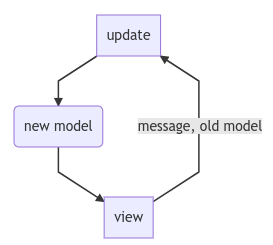
\includegraphics[width=\textwidth]{elm-architecture}
        \caption{The Elm Architecture}
        \label{fig:Figure 1}
    \end{subfigure}
    \begin{subfigure}[b]{0.2\textwidth}
        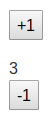
\includegraphics[width=0.3\textwidth]{counter}
        \centering
        \caption{Simple Counter App}
        \label{fig:Figure 2}
    \end{subfigure}
\end{figure}

\definecolor{codegray}{rgb}{0.5,0.5,0.5}
\lstset{numbers=right,numbersep=-10pt,numberstyle=\tiny\color{codegray}, language=Haskell}         
\begin{lstlisting}[caption={Elm Counter}]
type alias Model =
  { count : Int }
  
initialModel : Model
initialModel =
  { count = 0 }
 
type Msg
  = Increment
  | Decrement

update : Msg -> Model -> Model
update msg model =
  case msg of
    Increment ->
      { model | count = model.count + 1 }
    Decrement ->
      { model | count = model.count - 1 }
      
view : Model -> Html Msg
view model =
  div []
    [ button 
        [ onClick Increment ] 
        [ text "+1" ]
    , div 
        [] 
        [ text <| toString model.count ]
    , button 
        [ onClick Decrement ] 
        [ text "-1" ]
    ]

main : Program Never Model Msg
main =
  Html.beginnerProgram
    { model = initialModel
    , view = view
    , update = update
    }
\end{lstlisting}

The core of the architecture is its a compound state value, \lstinline{model}, \textbf{Listing 1, lines 1-6}. It represents the entirety of an applications state at any given time. Just like in imperative programming, the Elm Architecture is explicit only about the \textit{initial} values of the model, here defined in \textbf{Listing 1, line 6}. The reducer, \textbf{Listing 1, lines 12-18}, steps the model forward in response to messages, simulating a global bag of mutable variables that change over time. Messages are generated from events in the view \textbf{Listing 1, lines 20-32}, such as the \lstinline{Increment} and \lstinline{Decrement} messages, both from \lstinline{onClick} events.

\section{Reflex}

The Reflex library was built for Haskell web development via ghcjs, a Haskell to JavaScript compiler. It features higher-order and cyclic streams, which means that streams can contain streams, and streams can reference streams that reference themselves. It is these features that are necessary to maintain explicitness in FRP.

Like in traditional FRP\cite{elliott1997functional}, Reflex has two main concepts: Events and Behaviors. Events are discrete occurrences in time, while Behaviors are continuously defined values for all points in time. Reflex also has Dynamic values, which have the properties of Events and Behaviors, in they are defined in all points in time as well as emitting events at the discrete points in time when they change. In the following examples we use Events and Dynamics.

\begin{lstlisting}[{caption=Reflex Counter, keepspaces=true}]
button   :: Text -> m (Event ())
el       :: Text -> m a -> m a
display  :: Show a => Dynamic a -> m ()
(<$)     :: a -> Event b -> Event a
leftmost :: [Event a] -> Event a
foldDyn  :: (a -> b -> b) -> b -> Event a -> m (Dynamic b)

bodyElement :: MonadWidget t m => m ()
bodyElement = do
  rec evIncr <- button "+1"
    el "div" $ display count
    evDecr <- button "-1"
    count <- foldDyn (+) 0 $ leftmost 
      [  1 <$ evIncr
      , -1 <$ evDecr
      ]
  return ()
  
main :: IO ()
main = mainWidget bodyElement
\end{lstlisting}

Reflex uses \lstinline{do} syntax to lay out the order of HTML elements. In \textbf{Listing 2, line 10 and 12}, we create buttons with text \lstinline{"+1"} and \lstinline{"-1"}, and bind their click event streams of type \lstinline{Event ()} to the names \lstinline{evIncr} and \lstinline{evIncr}, respectively. Notice that in \textbf{Listing 2, line 11} \lstinline{count} is used before it is defined. In Reflex, statements are arranged vertically in the order in which they appear in the HTML DOM tree, not in the order they are "evaluated." There is no explicit evaluation order here. Instead this \lstinline{do rec} syntax allow us to set up an event propagation network \textit{at the same time} as we lay our our HTML elements. To calculate the \lstinline{count} from the button click events, we use

\begin{itemize}
\item \lstinline{<$} to map each click event to either \lstinline{1} or \lstinline{-1}, 
\item \lstinline{leftmost} (which is thusly named because in the case when events occur simultaneously -- which is impossible in this example because only one button can be clicked at a time -- it chooses only the event leftmost in the list) to merge the two event streams into a single event stream, and
\item  \lstinline{foldDyn (+)} to sum them up. 
\end{itemize}

However this architecture does not properly scale. For example, say we wanted to be able to set the value of the counter to a specific value, say another Dynamic, \lstinline{dynNum1}, in response to a third button press. Instead of summing of \lstinline{Event Int}, we can step forward the previous value of state with \lstinline{Event (Int -> Int)}. In Haskell \lstinline{($) :: (a -> b) -> a -> b} represents functional application, so here it applies each event function to the previous value of count.

\lstset{numbers=none}
\begin{lstlisting}
    count <- foldDyn ($) 0 $ leftmost 
      [ (+   1)         <$ evIncr
      , (+ (-1))        <$ evDecr
      , (\_ -> dynNum1) <$ evSet 
      ]  
\end{lstlisting}

This pattern is similar to the Elm Architecture in that it is a reduction over events. However this is a local reduction solely for this piece of state. If there were other independent pieces of state in this application, they would have separate reductions.

Even in this small example we can see how \lstinline{count} is defined more explicitly than in Elm. If we wish to understand how \lstinline{count} behaves, we have a singular place to look for what it depends upon, \lstinline{evIncr} and \lstinline{evDecr}, and precisely how, mapping them to \lstinline{(+ 1)} and \lstinline{(+ (-1))}, respectively, and then merging and applying. We will see the benefits more clearly in a larger example.

The price we pay for this explicitness is that events are abstracted from the single messages in Elm into streams of values. In Elm we write a global state reducer function that pattern matches on these event messages. In Reflex we use stream combinators to define the model and view as streams of each other. The single global I/O cycle of Elm becomes a number of cyclic definitions between model and view streams in Reflex.

\section{TodoMVC Comparison}

TodoMVC has become a standard application to compare front-end frameworks. It runs ~300 lines in both Elm and Reflex. We compare Elm ToDoMVC \footnote{https://github.com/evancz/elm-todomvc/blob/master/Todo.elm} with Reflex ToDoMVC \footnote{https://github.com/reflex-frp/reflex-todomvc/blob/develop/src/Reflex/TodoMVC.hs}. Say we wish to understand the behavior of the list of todo items in both implementations.\newline

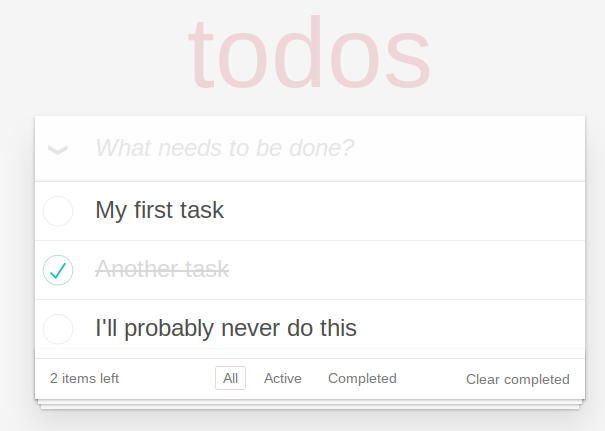
\includegraphics[width=0.35\textwidth]{todomvc}\newline

\subsection{Elm TodoMVC}

In Elm, any message can modify any state. For example, in \lstinline{update},  the \lstinline{Add} message triggers an update of three different pieces of state:

\begin{lstlisting}
Add ->
  { model
    | uid = model.uid + 1
    , field = ""
    , entries = if String.isEmpty model.field then model.entries else model.entries ++ [ newEntry model.field model.uid ]
  }
\end{lstlisting}

Thus there is no single place to look to understand how the todo items list, here called  \lstinline{entries}, behaves. We must Ctl-F for all occurrences of  \lstinline{entries =} as seen in \textbf{Fig. 2}.

\begin{figure}[h]
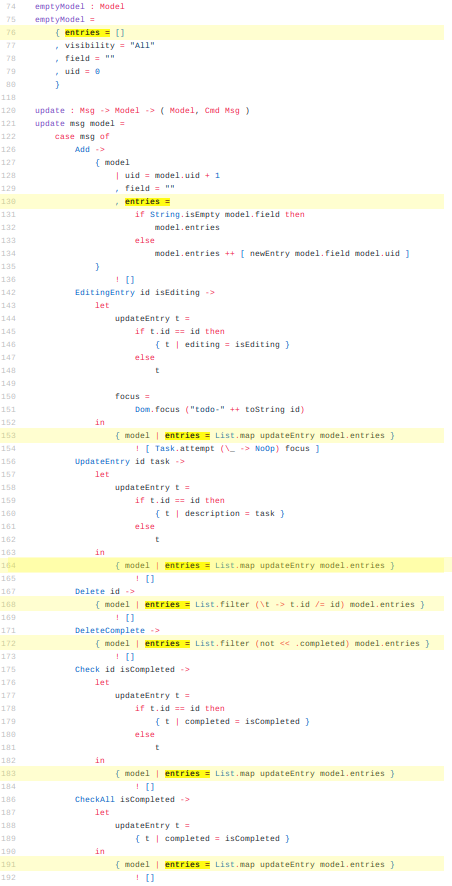
\includegraphics[scale=0.35]{elm-entries}
\caption{Elm TodoMVC entries modifications highlighted in reducer}
\label{fig:figure 2}
\end{figure}

In other words, we cannot gain a complete understanding of any piece of state by looking in one place. We have to look through \textit{all} messages to see if it affects the state in question, and then piece together \textit{in our head} how the sum total of these effects come together to form an integrated behavior. In this way, the Elm Architecture's reducer simulates the "primitive word-at-a-time style of programming inherited from the von Neumann computer ... instead of encouraging us to think in terms of the larger conceptual units of the task at hand."\cite{Backus:1978:PLV:359576.359579}

There's also a subtler way the Elm Architecture undermines explicitness: each piece of state can be modified in terms of \textit{any other piece of state}. There's no explicit isolation between independent states. 

Next, any view element can emit any number of messages. We know from our Ctl-F above that the \lstinline{Add}, \lstinline{EditingEntry}, \lstinline{UpdateEntry}, \lstinline{Delete}, \lstinline{DeleteComplete}, \lstinline{Check}, and \lstinline{CheckAll} events can affect \lstinline{entries}, so now we Ctl-F for each of those events to see which HTML elements emit those messages in response to which events as seen in \textbf{Fig. 3}. 

\begin{figure}[h]
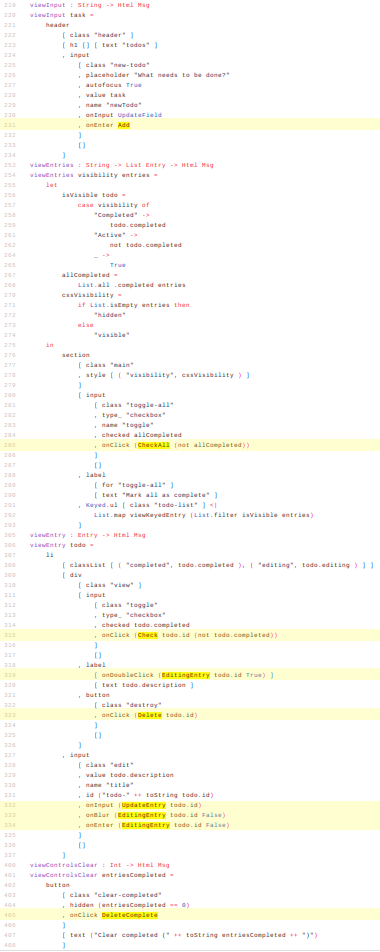
\includegraphics[scale=0.35]{elm-actions}
\caption{Elm TodoMVC relevant actions highlighted in view}
\label{fig:figure 3}
\end{figure}

If we're looking to understand a single piece of state in Elm, we're not much better off than with an entirely imperative framework: we still have to read more-or-less the whole application even if we wish only to comprehend only a small piece. Explicitness is lost as surely as if we passed around a compound state value to all of our functions, which is in fact what we've done.

\subsection{Reflex TodoMVC}

By contrast, if we wish to understand the same piece of state in Reflex's TodoMVC, there is a single explicit place to look, \textbf{Listing 3, lines 16-19}. This definition uses the more scalable pattern we discussed for the counter application above. There we had \lstinline{Event (Int -> Int)} and here we have \lstinline{Event (Map Int Task -> Map Int Task)}. Here \lstinline{tasks} is a merging of three events:

\begin{enumerate}
\item \lstinline{fmap insertNew_ newTask} is where new tasks are added to the list.
\item \lstinline{listModifyTasks} handles the vast majority of task mutations, including deletions, completions (and their reversal), and task text editing. This definition depends on \lstinline{tasks} and \lstinline{activeFilter}.
\item \lstinline{fmap (const $ Map.filter $ not . taskCompleted)}  \newline \lstinline{clearCompleted} filters out the currently-completed tasks all at once when the "Clear Completed" button is clicked.
\end{enumerate}

\begin{lstlisting}[{caption=Elm TodoMVC,numbers=right}]
initialTasks :: Map Int Task
initialTasks = Map.empty

insertNew_ :: Task -> Map Int Task -> Map Int Task

todoMVC :: ( DomBuilder t m
           , DomBuilderSpace m ~ GhcjsDomSpace
           , MonadFix m
           , MonadHold t m
           )
        => m ()
todoMVC = do
  el "div" $ do
    elAttr "section" ("class" =: "todoapp") $ do
      mainHeader
      rec tasks <- foldDyn ($) initialTasks $ mergeWith (.)
            [ fmap insertNew_ newTask
            , listModifyTasks
            , fmap (const $ Map.filter $ not . taskCompleted) clearCompleted
            ]
          newTask <- taskEntry
          listModifyTasks <- taskList activeFilter tasks
          (activeFilter, clearCompleted) <- controls tasks
      return ()
    infoFooter
\end{lstlisting}

Explicitness allows us to see the shape of this application and how its pieces come together to make an integrated whole. We see where code is independent, such as \lstinline{taskEntry}, and dependent, such as \lstinline{tasks} on \lstinline{activeFilter}. If we only cared about one piece of behavior and its associated interface, we could rely on this explicit independence to safely ignore the others. In \textbf{Fig. 7}, we can see the explicit relationships between Reflex TodoMVC's Dynamics and HTML elements that are obfuscated in Elm TodoMVC \textbf{Fig. 6}.

\section{Is the cure worse than the disease?}

This paper argues for higher-order and cyclic streams for the purposes of \textit{comprehensibility}. Yet the dense Reflex code and diagram don't seem easy to understand. The creator of Elm takes this stance, arguing that explicit dependencies lead to a "crazy" graph of dependencies\footnote{https://youtu.be/DfLvDFxcAIA?t=27m32s}.

The Elm Architecture has many benefits. For one, it simulates global mutable state, which is very familiar to most programmers. The one-message-at-a-time style does simplify the code writing process. It also reduces coupling between the view and the model. Finally, Elm's model variable is easily serialized, which allows for time-travel debugging, hot reloading, and easy-to-implement undo features.

While it is easier to \textit{write} in the Elm Architecture in a small application, we are concerned with the more common case of navigating a large application one does not know well. Here the Reflex diagram in \textbf{Fig. 7} shines by showing how the application fits together, and what we need to read.

The Elm Architecture reduces coupling, but there can be too little coupling. The amount of coupling in code should reflect the essential coupling in the underlying idea. If the nature of an interface is cyclic, the code shouldn't obfuscate that fact, but expose it clearly. More importantly it should make explicit the independence of independent entities.

To be fair, let's not understate the difficulty of writing Reflex code. It is hell on earth, grappling with its unwieldy types, double \lstinline{fmap}ing over streams, and waiting for \lstinline{ghcjs} to compile. Reflex is a reasonably sound computational model that is in much need of a interface upgrade, discussed further in \textbf{Section 7}.

\section{Related work}

The field of program slicing\cite{slicing} takes a different approach to the problem of code dependencies. It leaves the underlying imperative programming model the same, and uses both static analysis and execution traces to determine which sections of code are relevant. 

It may be possible to keep the simpler semantics of the Elm Architecture, and generate interdependencies via static analysis. In Elm, accessing and modifying records can only be done with static keys, so we can determine exactly which messages modify which pieces of state, which view elements depend on which pieces of state, and which view elements emit which messages. Potentially we'd be able to generate a graph as pleasing as \textbf{Fig. 7} with Elm. However this static analysis would be much less powerful in Elm-Architecture-inspired JavaScript frameworks (Redux or VueX), because in JavaScript one can access objects with dynamic string keys, so it'd be difficult to be sure what's accessed and modified where.

\section{Future work}

\subsection{Visualizations}

While the Reflex library's semantics are ideal for modular comprehensibility, the library itself is difficult to use. For one, the syntax is difficult to parse. Given that our goal is comprehensibility, this is unacceptable. I am inspired by the visual stream combinators of RxMarbles\footnote{http://rxmarbles.com/} (\textbf{Fig. 4}).

\begin{figure}[h!]
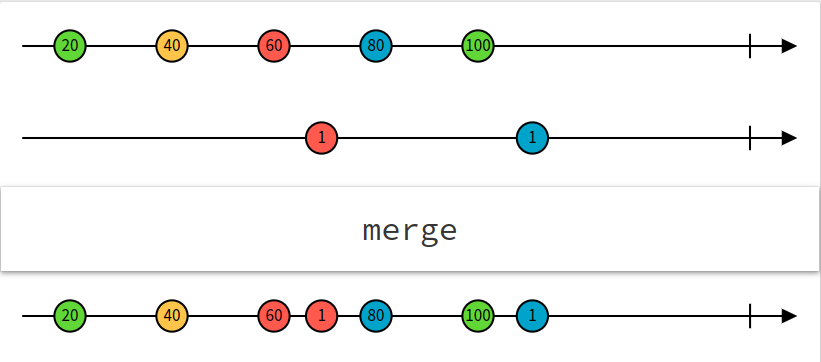
\includegraphics[scale=0.2]{rxmarbles}
\caption{RxMarbles}
\label{fig:figure 4}
\end{figure}

RxViz\footnote{https://rxviz.com/} and RxFiddle\footnote{https://rxfiddle.net} parse streams from code and visualize them dynamically. RxViz does a particularly good job of visualizing the evolution of higher-order streams in realtime. However, RxViz only shows the final output stream, not how the various input streams combine. RxFiddle makes an effort to show the high-level view of stream dependencies (in \textbf{Fig. 5} between the code and marble diagrams).

\begin{figure}[h!]
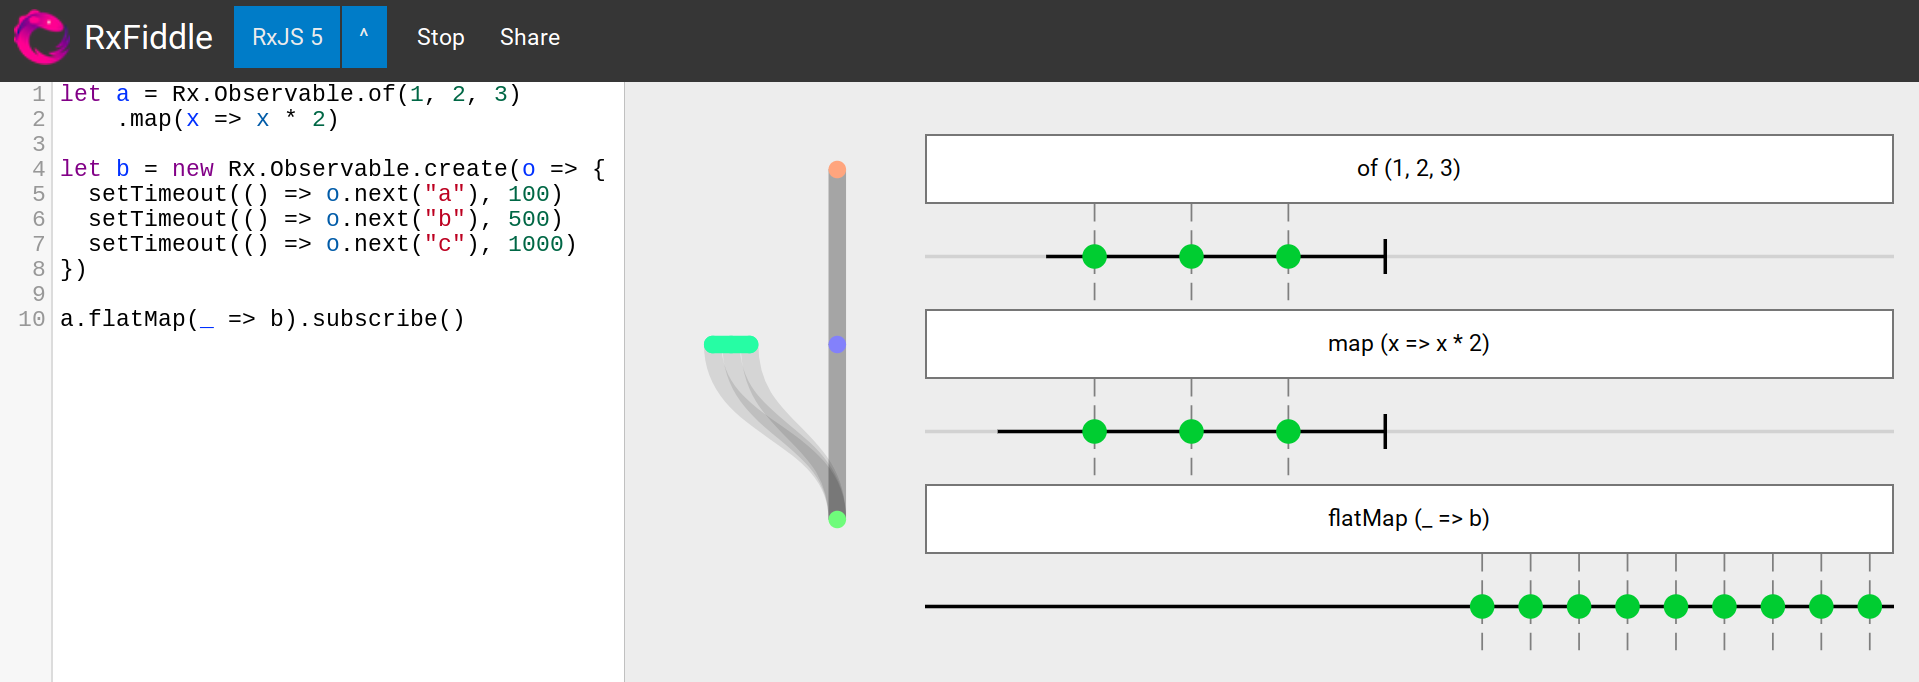
\includegraphics[width=0.4\textwidth]{rxfiddle}
\caption{RxFiddle}
\label{fig:figure 5}
\end{figure}

One challenge in particular will be visualizing cyclic dependencies. This may require learning from M. C. Escher.

Eventually, it would be ideal if one could edit the streams from the visual representation directly.

\subsection{JavaScript-based}

It order to be a true alternative to the Elm Architecture in the broader JavaScript community, a competing model must be performant in JavaScript. In theory, it is possible to create a cyclic event propagation network (to copy Reflex's implementation) in JavaScript, but JavaScript's semantics are quite different from pure functional programming so it may not have a natural feel.  The CycleJS library\footnote{https://cycle.js.org/} allows for higher-order, and even semi-cyclic streams\footnote{https://github.com/staltz/xstream\#-imitatetarget}, so maybe it wouldn't be difficult. 

\section{Conclusion}

As the popularity of FRP frameworks continues, it's increasingly important to have a data model architecture that prioritizes the comprehensibility of large programs. This paper does not present a direct solution to this problem, but instead attempts to sound the alarm that what we're currently satisfied with, The Elm Architecture, is not good enough. The Reflex library, with its higher-order and cyclic streams, points in the right direction, but we are still far from a complete solution to the problem of comprehensible user interface construction.

\bibliographystyle{ACM-Reference-Format}
\bibliography{frp.bib}

\begin{figure*}[pt]
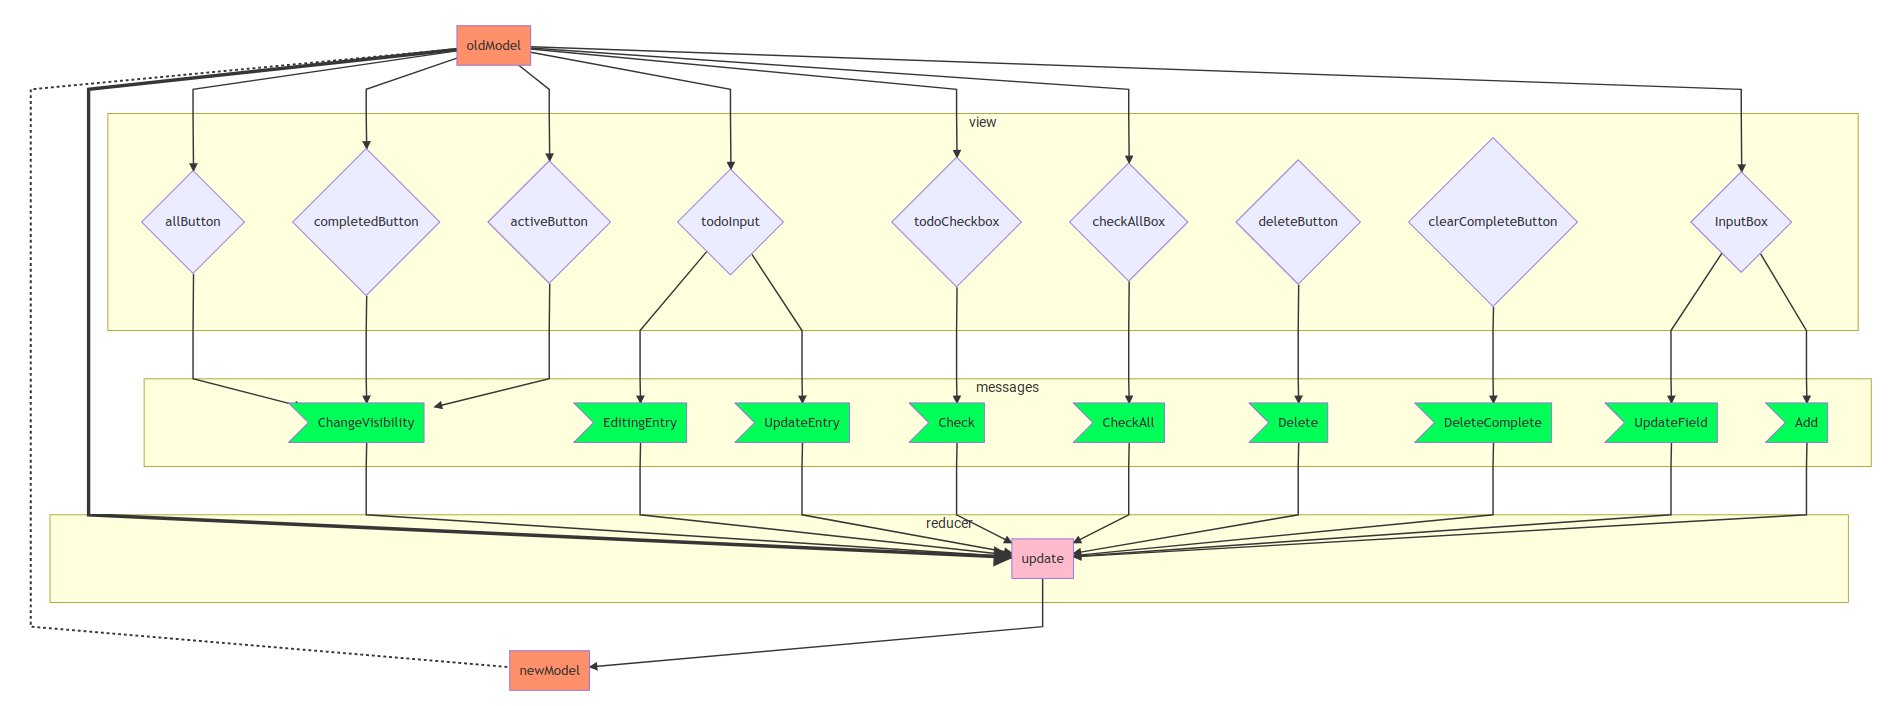
\includegraphics[width=0.8\textwidth]{elm-graph}
\centering
\caption{Elm TodomMVC Diagram. HTML elements are rotated blue squares. Messages are green and rectangular. All messages point to the pink reducer, which point to the newModel, which is linked to the oldModel at the top via a dotted line.}
\label{fig:figure 6}
% TODO include description
\end{figure*}

\begin{figure*}[pb]
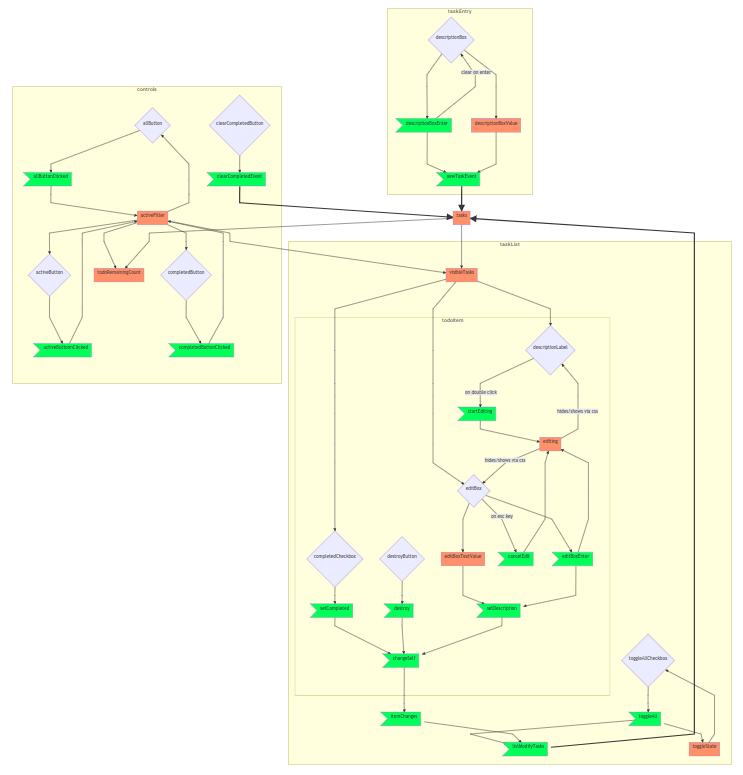
\includegraphics[width=0.73\textwidth]{reflex-graph}
\caption{Reflex TodomMVC Diagram. The top-level tan categories represent widget definitions. HTML elements are rotated blue squares, Events are green rectangles, missing a triangle, and Dynamics are orange rectangles. The three arrows for the three dependencies of \lstinline{tasks} are bold.}
\label{fig:figure 7}
\end{figure*}



\end{document}
